\section{Extensive test in car environment}
To perform a real-life use case test, we set up a complete data-acquisition system composed of:
\begin{itemize}
    \item All the seven sensor boards of this thesis: 2 ST SensorTile.box, 2 ST BlueTile, 3 MBIENTLAB MetaMotionS.
    \item A SONY Action Cam HDR-AS200V, to match recorded data with video information. As the device contains a GPS module, also localization information is recorded. 
    \item A smartphone equipped with the Physics Toolbox application, used to sample reference data from accelerometers, gyroscope and GPS sensors.
    \item A device from Tierra SpA with high-precision IMU sensors and a GPS module. 
\end{itemize}

The data collection phase lasted for about one hour, in which we went through different paths around the Politecnico di Torino, including roundabouts, different round surfaces and start/stop conditions. Every particular condition have been signaled with precise audio frequencies, generated by another smartphone with the Physics Toolbox application and reported in Table \ref{audio-freq}. Figure \ref{fig:ex1map} shows a map of the road traveled for the experiment, while Figure \ref{fig:sensors_positioning} reports the setup of the sensors inside the car. 

\begin{figure}[ht!]
        \centering
        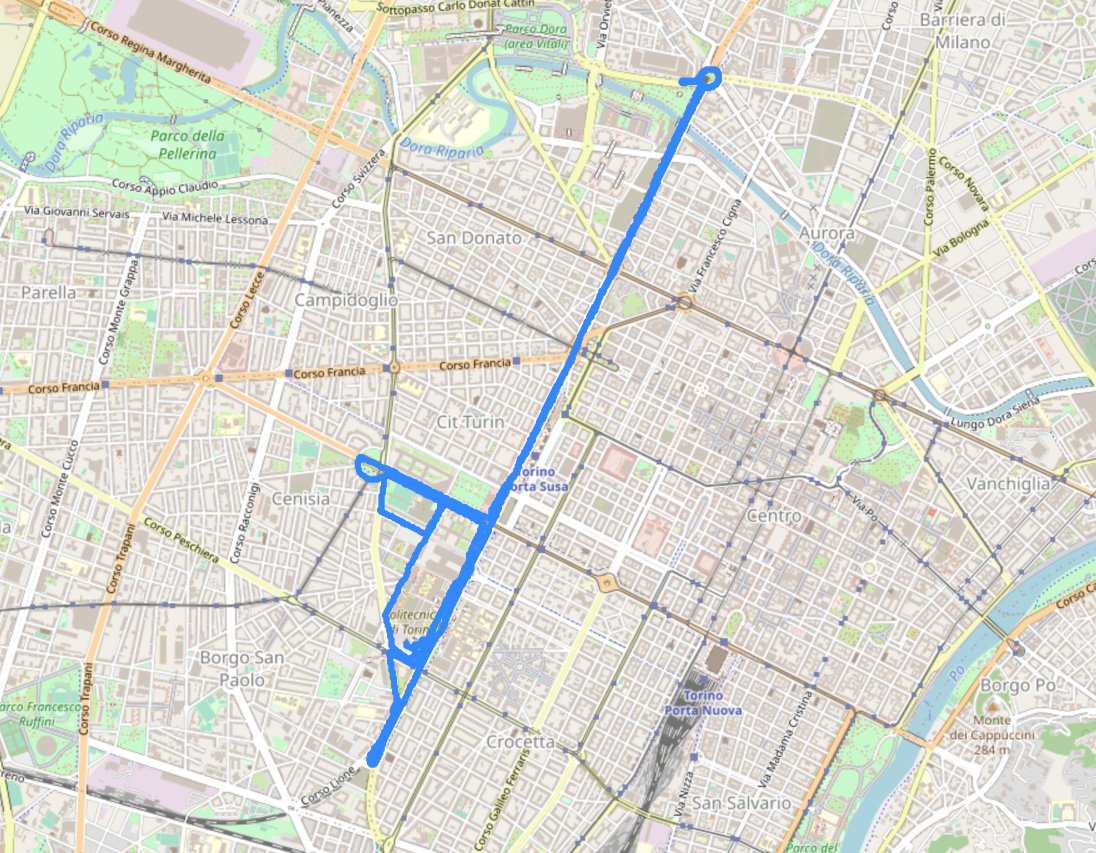
\includegraphics[width=0.75\textwidth]{chap4/figure/map.png}
        \caption{Map of the road traveled for the car experiment (OpenStreetMap).}
        \label{fig:ex1map}
\end{figure}

\begin{table}[ht!]
\centering
\caption{Car experiment: events and corresponding audio frequency.}
\begin{tabular}{|c|c|}
\hline
\textbf{Event}            & \textbf{Sound Frequency (Hz)} \\ \hline
Experiment start          & 400                           \\ \hline
Roundabout                & 800                           \\ \hline
Road bump (long)          & 1200                          \\ \hline
Road bump (short)         & 1600                          \\ \hline
Start from traffic light  & 2000                          \\ \hline
Braking for traffic light & 2400                          \\ \hline
Right turn                & 2800                          \\ \hline
Left turn                 & 3200                          \\ \hline
\end{tabular}
\label{audio-freq}
\end{table}

\FloatBarrier

\begin{figure}[hbtp]
        \centering
        \subfigure[First SensorTile.box on the right of the car dashboard]
            {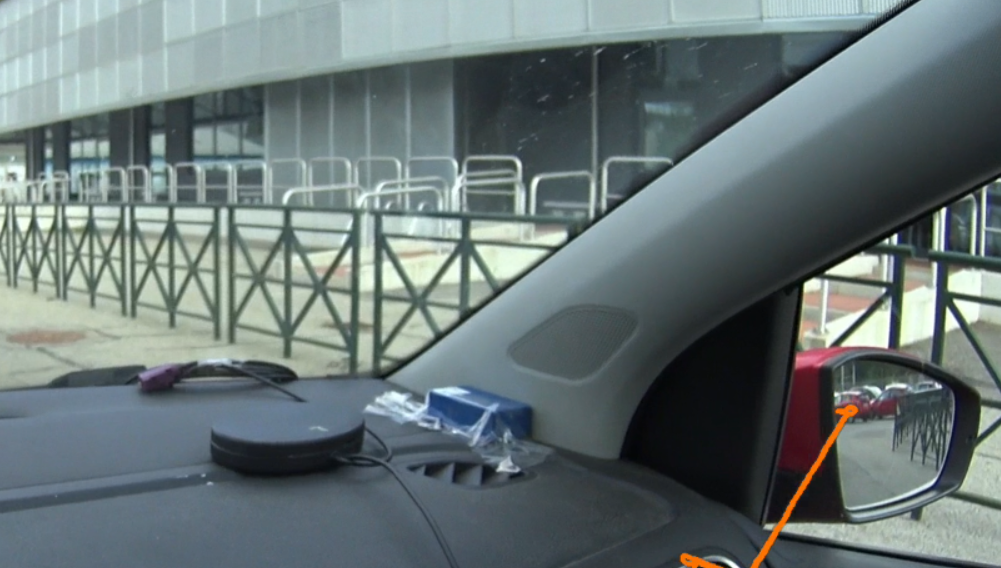
\includegraphics[width=0.45\textwidth]{chap4/figure/position_st1.png}}
        \hspace{5mm}
        \subfigure[Second SensorTile.box on the left of the car dashboard]
            {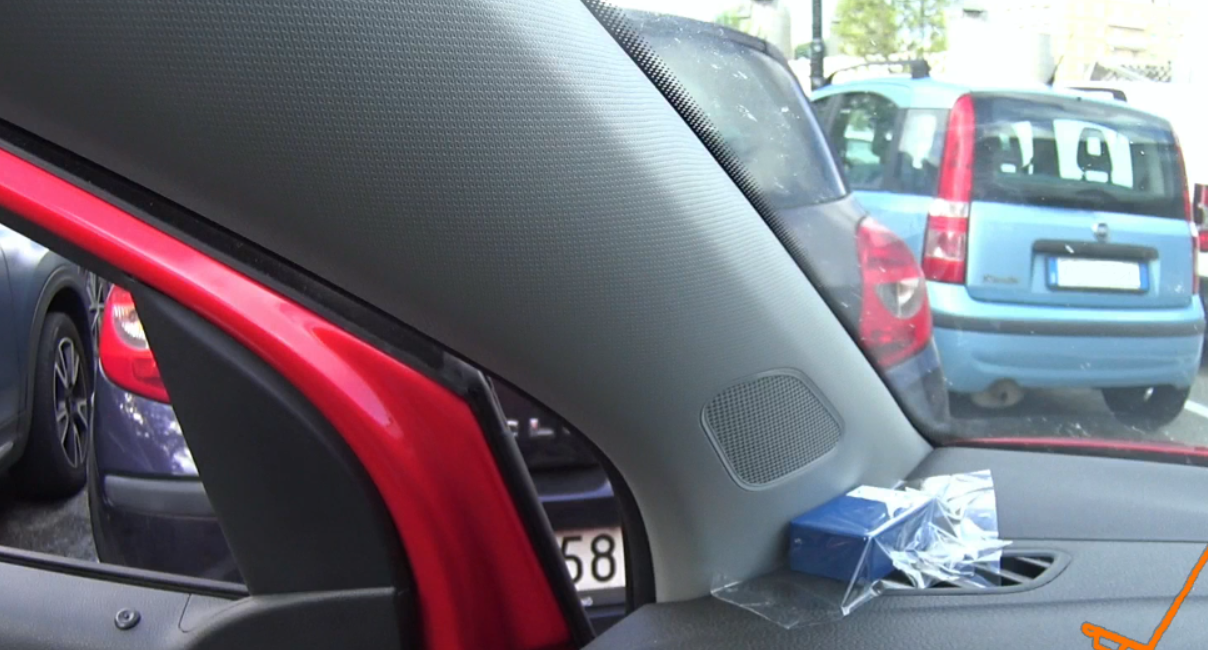
\includegraphics[width=0.45\textwidth]{chap4/figure/position_st2.png}}      
        \hspace{5mm}
        \subfigure[BlueTile and BlueVoice boards on the center of the car dashboard]
            {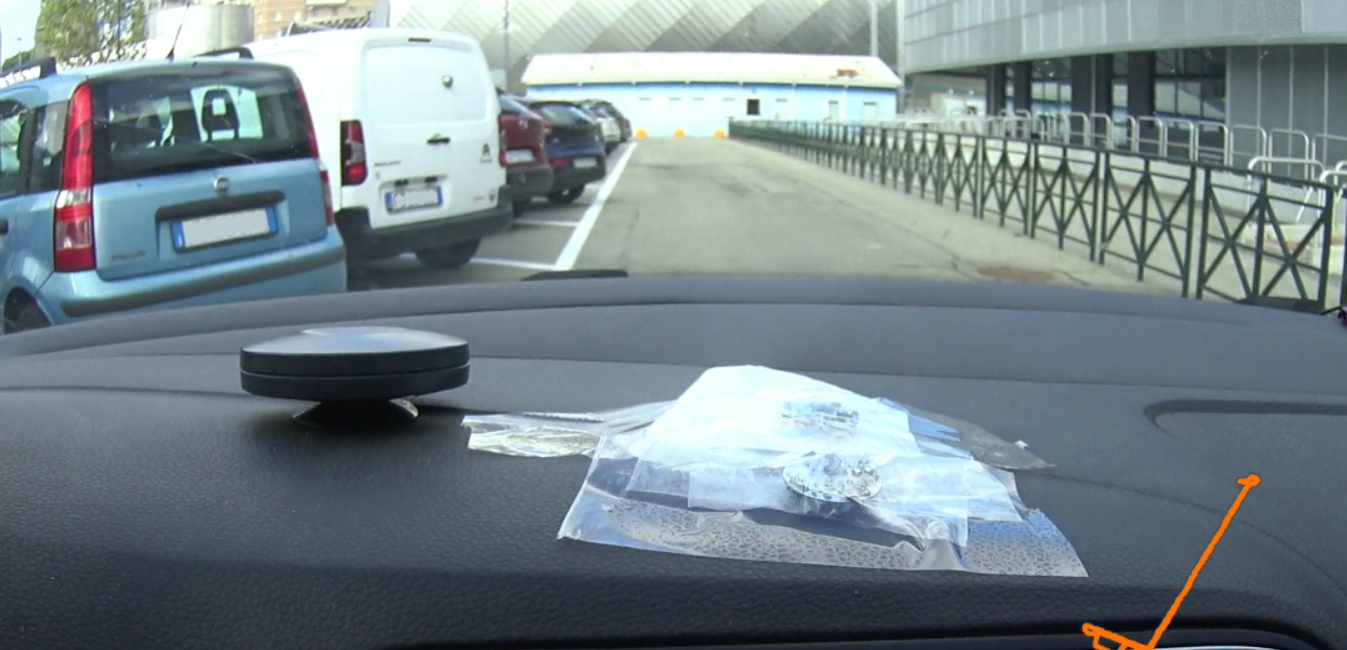
\includegraphics[width=0.45\textwidth]{chap4/figure/position_bv.png}}
        \hspace{5mm}
        \subfigure[One MetaMotion fixed on the driver's seat]
            {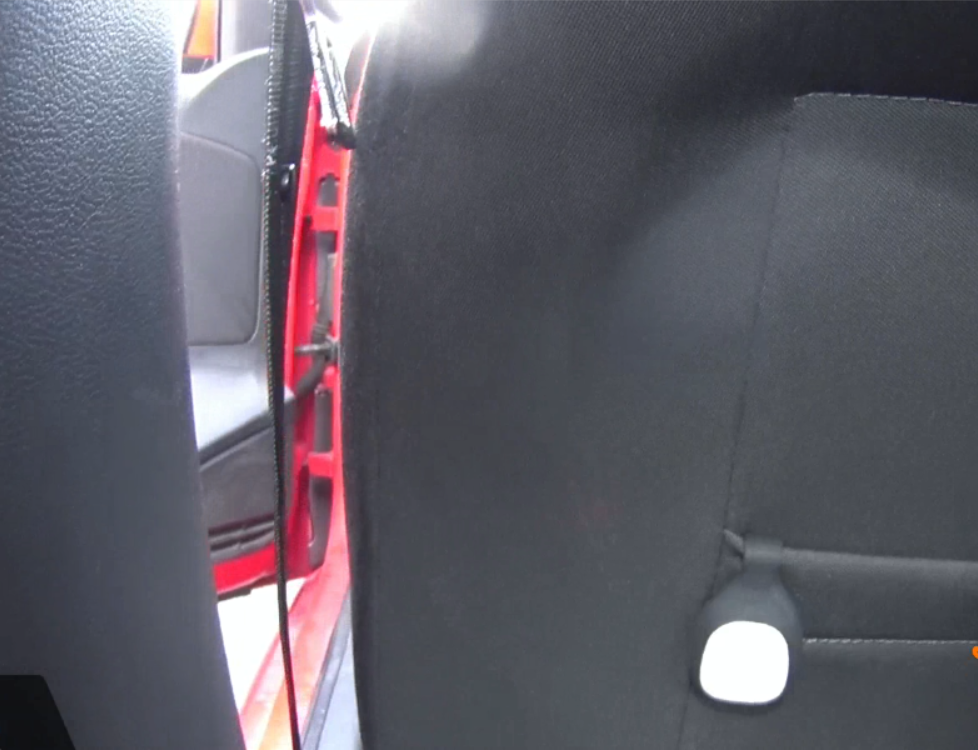
\includegraphics[width=0.45\textwidth]{chap4/figure/position_mm1.png}}
        \hspace{5mm}
        \subfigure[One MetaMotion fixed on the passenger's seat, with the Tierra device]
            {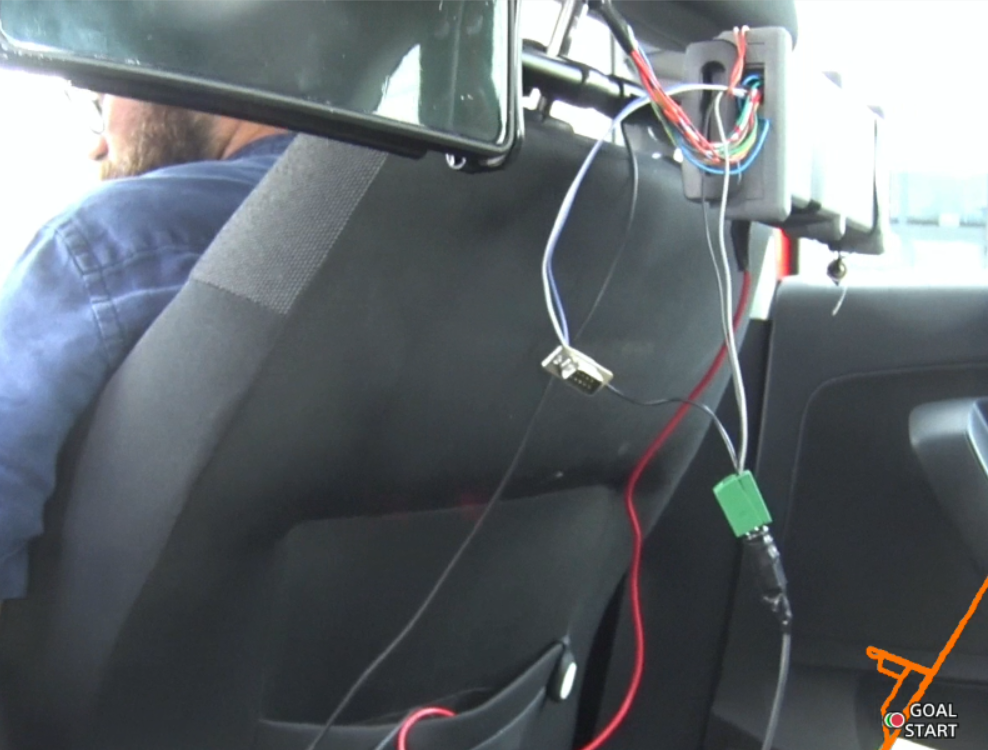
\includegraphics[width=0.45\textwidth]{chap4/figure/position_mm2.png}}
        \hspace{5mm}
        \subfigure[One MetaMotion fixed on the belt of a rear seat]
            {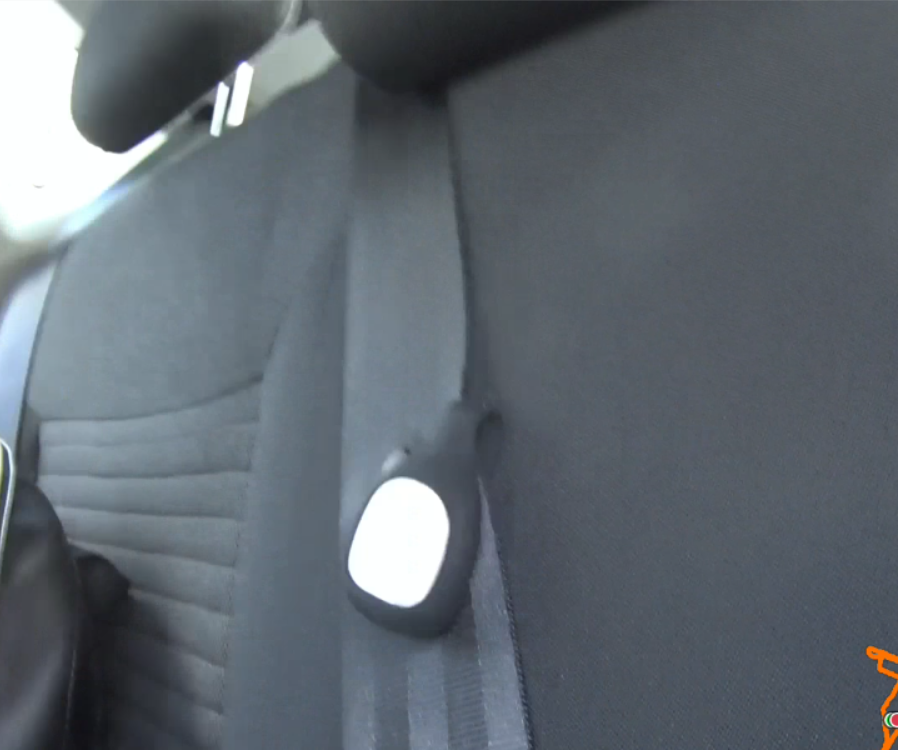
\includegraphics[width=0.45\textwidth]{chap4/figure/position_mm3.png}}
        \caption{Images of the positioning of the sensor boards in the car.}
        \label{fig:sensors_positioning}
\end{figure}
\newpage

As results, I'm reporting in the following figures the graphs obtained by considering both the acceleration and the gyroscope data. 

 Figure \ref{fig:car-overall-acc} reports acceleration data coming from all the sensors. I reported the X axis for ST sensors (x1, x2, x3), and Z axis for MetaMotionS sensors (mz1, mz2, mz3). In this way, the direction plotted is the same for all sensors: in the way they were mounted, axis X for ST devices coincided with axis Z of the other ones when compared to the car movement.  
\begin{figure}[ht!]
        \centering
        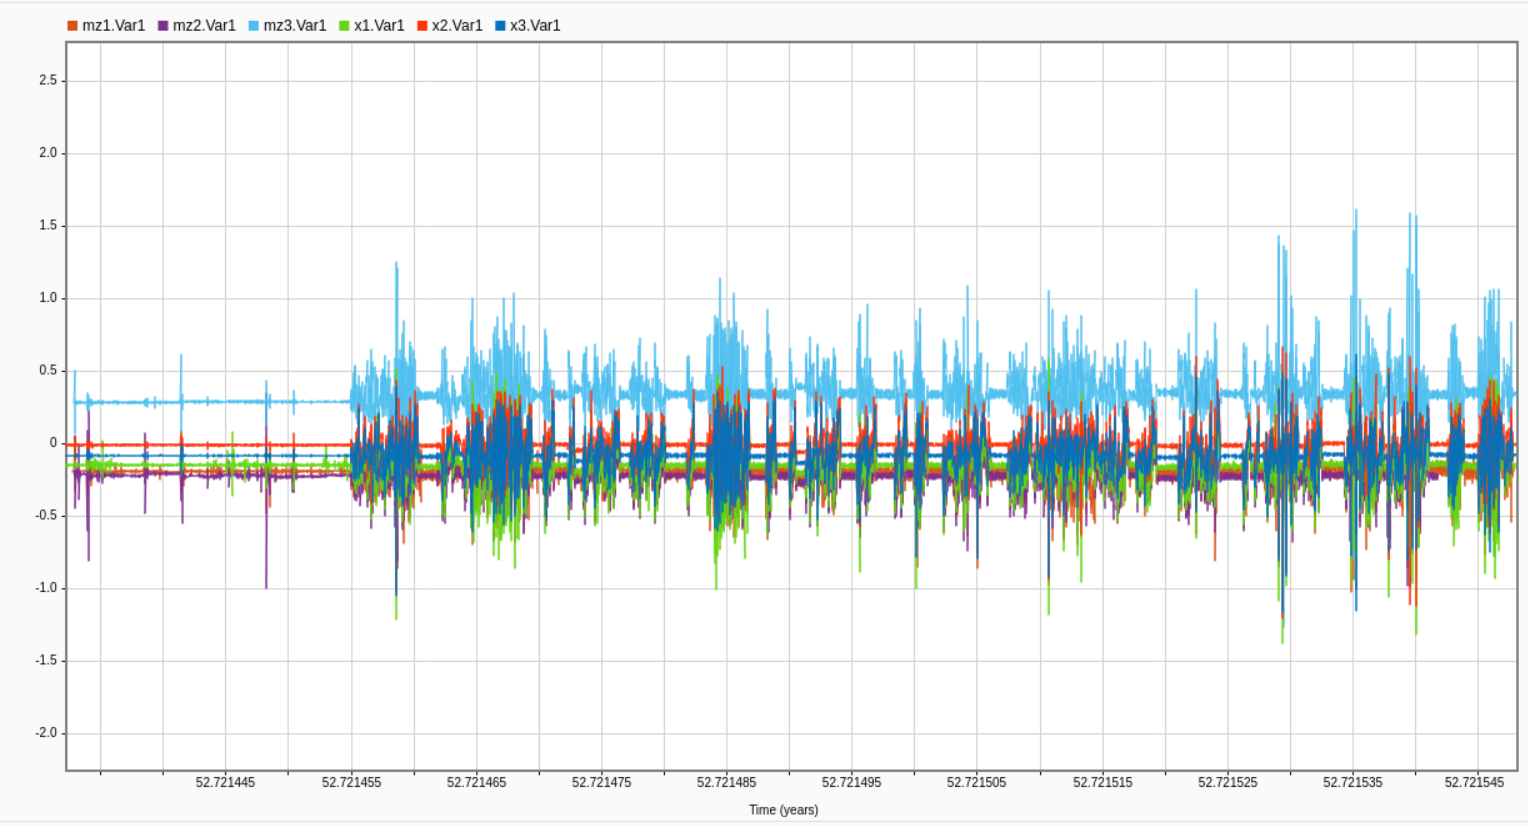
\includegraphics[width=0.85\textwidth]{chap4/figure/car_test_overall_acc.png}
        \caption{Graph representing acceleration on the X axis for all the sensor boards.}
        \label{fig:car-overall-acc}
\end{figure}

Figure \ref{fig:car-detail1-acc} represents data for a particular acceleration event that happened in the last part of sampling. From this, I noticed that a MetaMotionS (mz3, light blue) is providing data differently from the other ones: it is the one mounted on the rear seat belt. First, it is 180° rotated (the front of this sensor board is facing the windscreen, while other ones are facing the rear window): hence, it is reporting data upside down. Then, it isn't perfectly perpendicular to the pavement, and a component of the gravity acceleration is generating an offset that is more evident than the one sensed by the other boards. 
\begin{figure}[ht!]
        \centering
        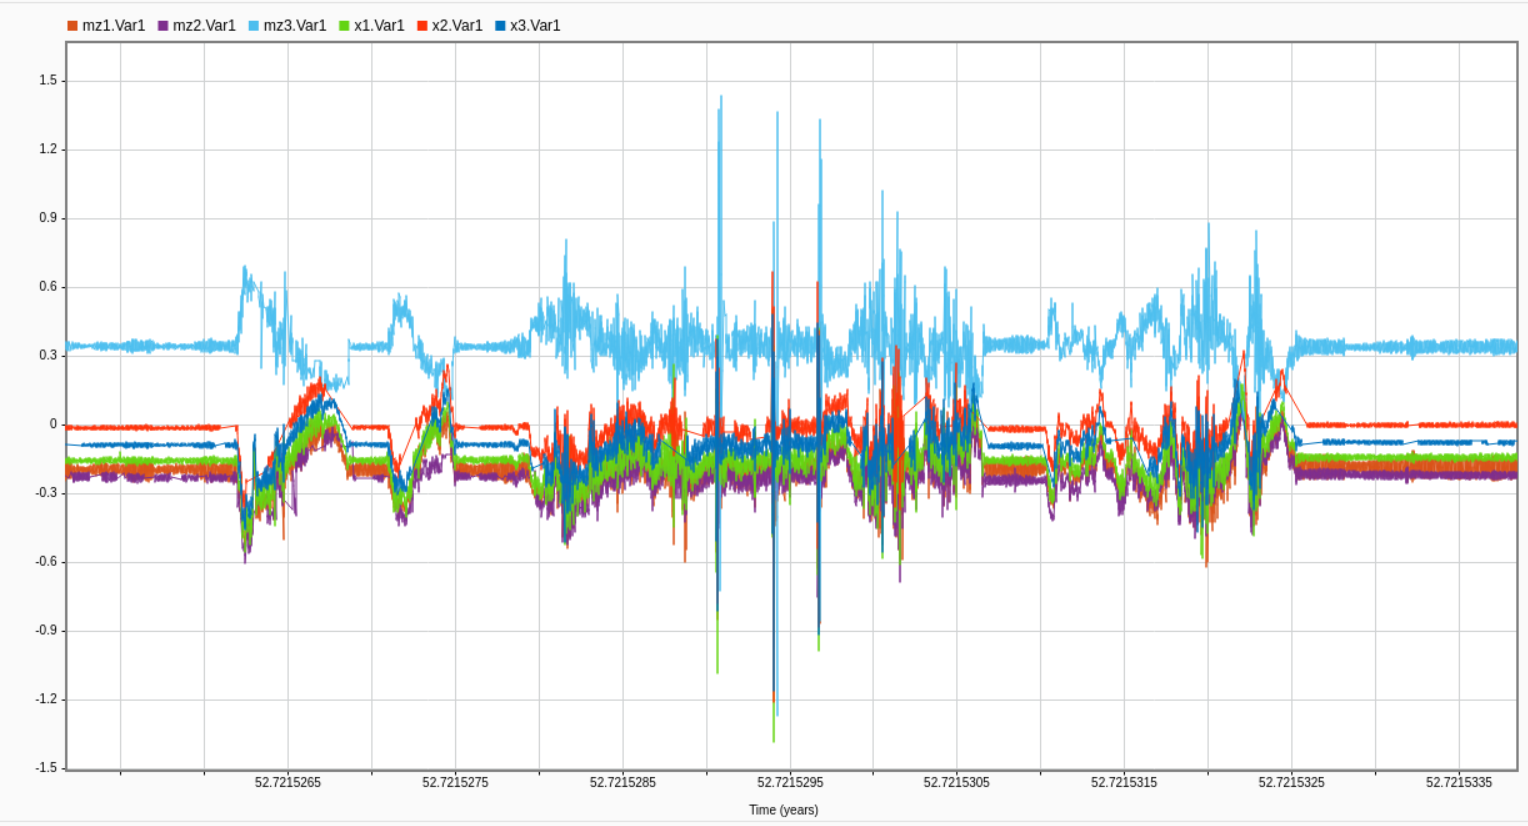
\includegraphics[width=0.85\textwidth]{chap4/figure/car_test_acc_detail1.png}
        \caption{Detail of acceleration in the minute domain.}
        \label{fig:car-detail1-acc}
\end{figure}

Figure \ref{fig:car-detail2-acc} shows acceleration samples in a smaller time interval. In particular, I wanted to represent the accuracy of time synchronization: the samples are taken from one of the final acceleration events of the experiment, but the peaks are still well aligned. Also in this case, the third MetaMotionS is behaving in an interesting way as its samples seems delayed. This seemed strange at first, because I tested the performances of MBIENTLAB time synchronization mechanism and it worked perfectly every time. I think that the motivation of the difference is due to the installation on the seat belt, that is not as stiff as the other points on which the sensors were put. 

\begin{figure}[ht!]
        \centering
        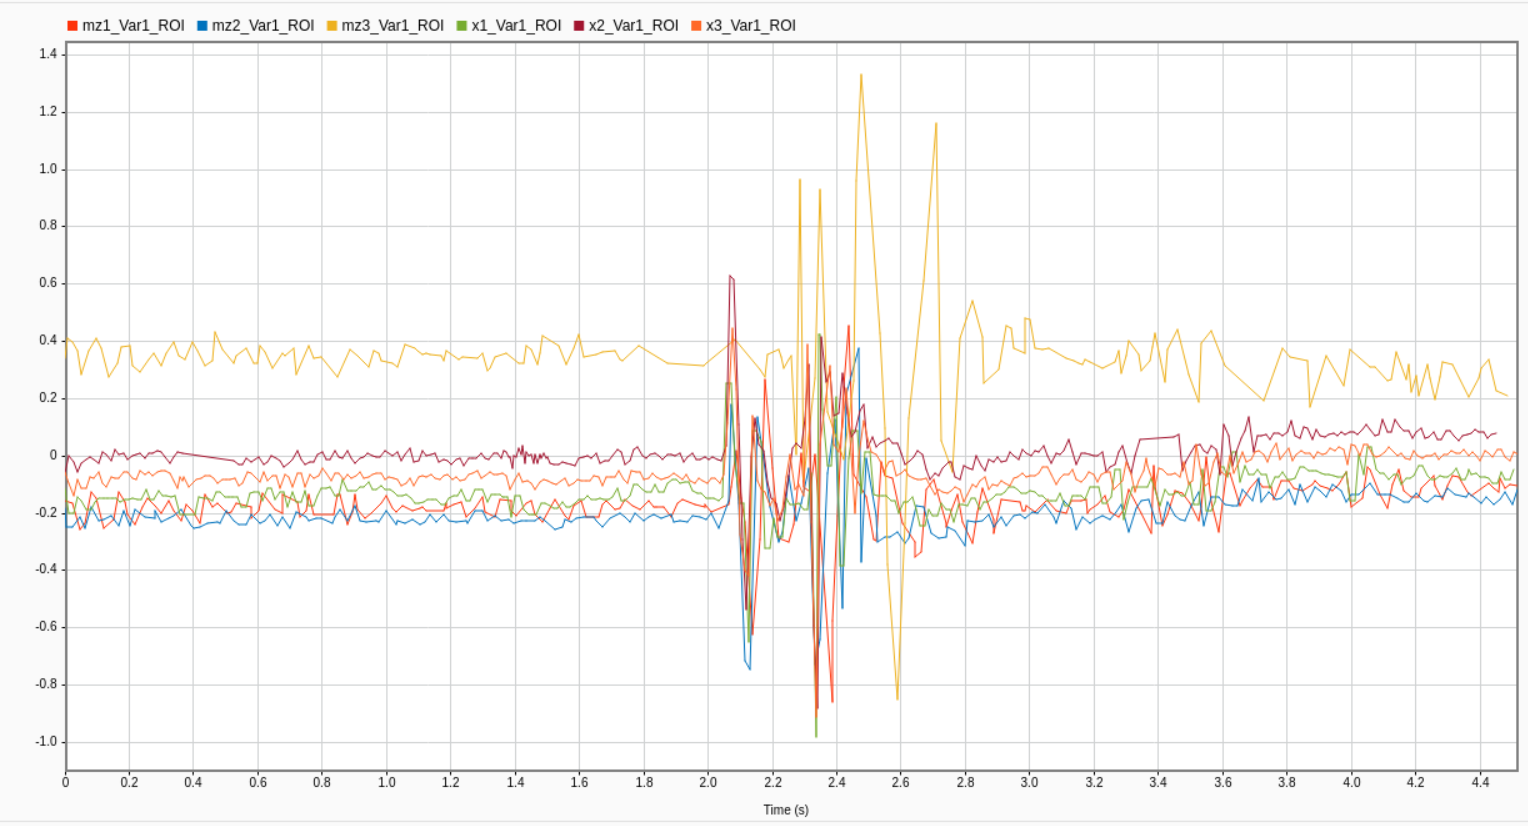
\includegraphics[width=0.85\textwidth]{chap4/figure/car_test_acc_detail2.png}
        \caption{Detail of acceleration in the seconds domain.}
        \label{fig:car-detail2-acc}
\end{figure}

Figure \ref{fig:car-overall-freqacc} is reporting the acceleration data from one of the sensor boards (in green) compared to the dominant value of the audio frequency for each instant (in light blue, dashed lines). To make the values comparable inside the same graph, the frequency values have been scaled: \(f_{GRAPH} = \frac{f_{ORIGINAL}}{1000}\). During the experiment, we played some frequencies more times with respect to what is shown here, so this was not the result I was expecting. 

\begin{figure}[ht!]
        \centering
        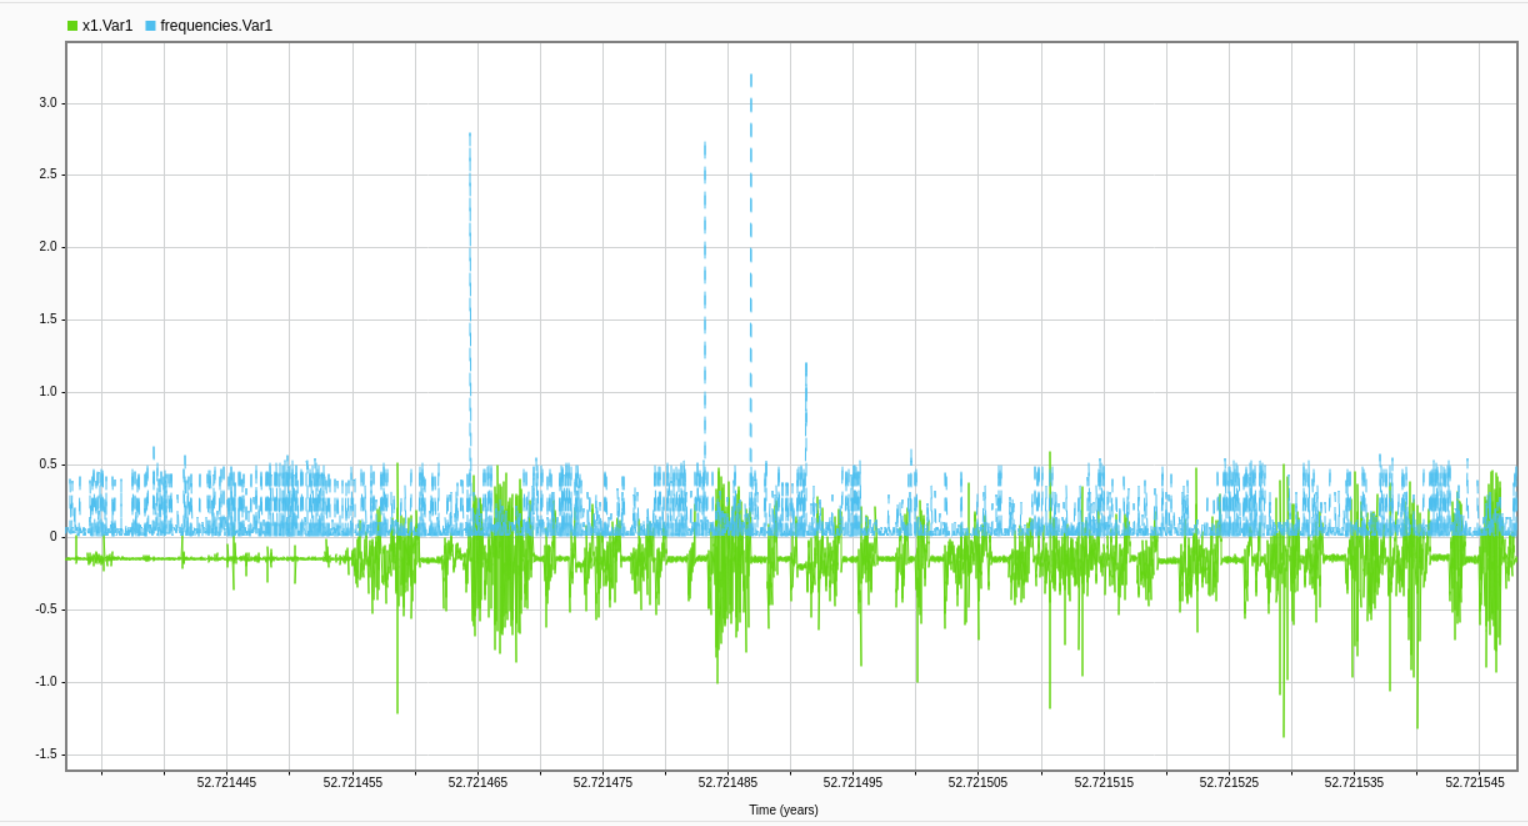
\includegraphics[width=0.85\textwidth]{chap4/figure/car_test_acc_frequencies.png}
        \caption{Graph of the acceleration data accompanied by audio frequency data.}
        \label{fig:car-overall-freqacc}
\end{figure}

Figure \ref{fig:car-detail-freqacc} reports two particular audio events, with an acceleration event between them. In particular, after the right turn tone (2.8~kHz), acceleration is present, and after the left turn tone (3.2~kHz), acceleration is 0 for some moments (probably because we were giving the right to pass at the intersection). Hence, the frequency analysis is working correctly, but some issues should be resolved. I'm discussing this later.

\begin{figure}[ht!]
        \centering
        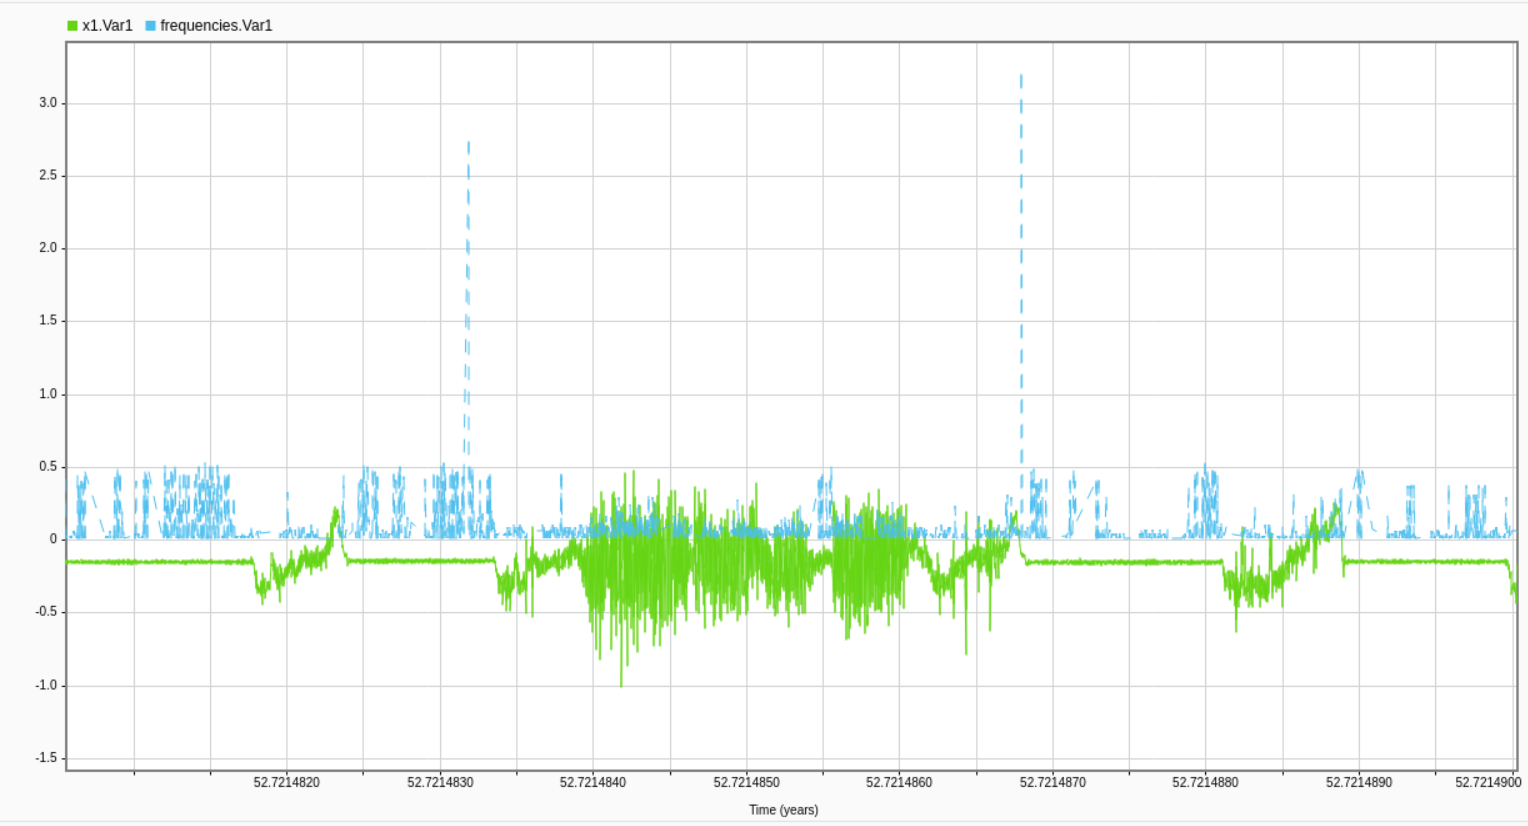
\includegraphics[width=0.85\textwidth]{chap4/figure/car_test_acc_frequencies_deatils.png}
        \caption{Graph of the acceleration data accompanied by audio frequency data, detail between two audio events.}
        \label{fig:car-detail-freqacc}
\end{figure}

Figures \ref{fig:car-overall-gyro} and \ref{fig:car-detail-gyro} represent the gyroscope data, both an overall view and a more detailed one. Also in this case, I noticed a different behaviour of the third MetaMotionS board, again because it's mounted on a seat belt and motion is transmitted differently. It is interesting to notice that these sensors are able to show this difference so precisely. 

\begin{figure}[ht!]
        \centering
        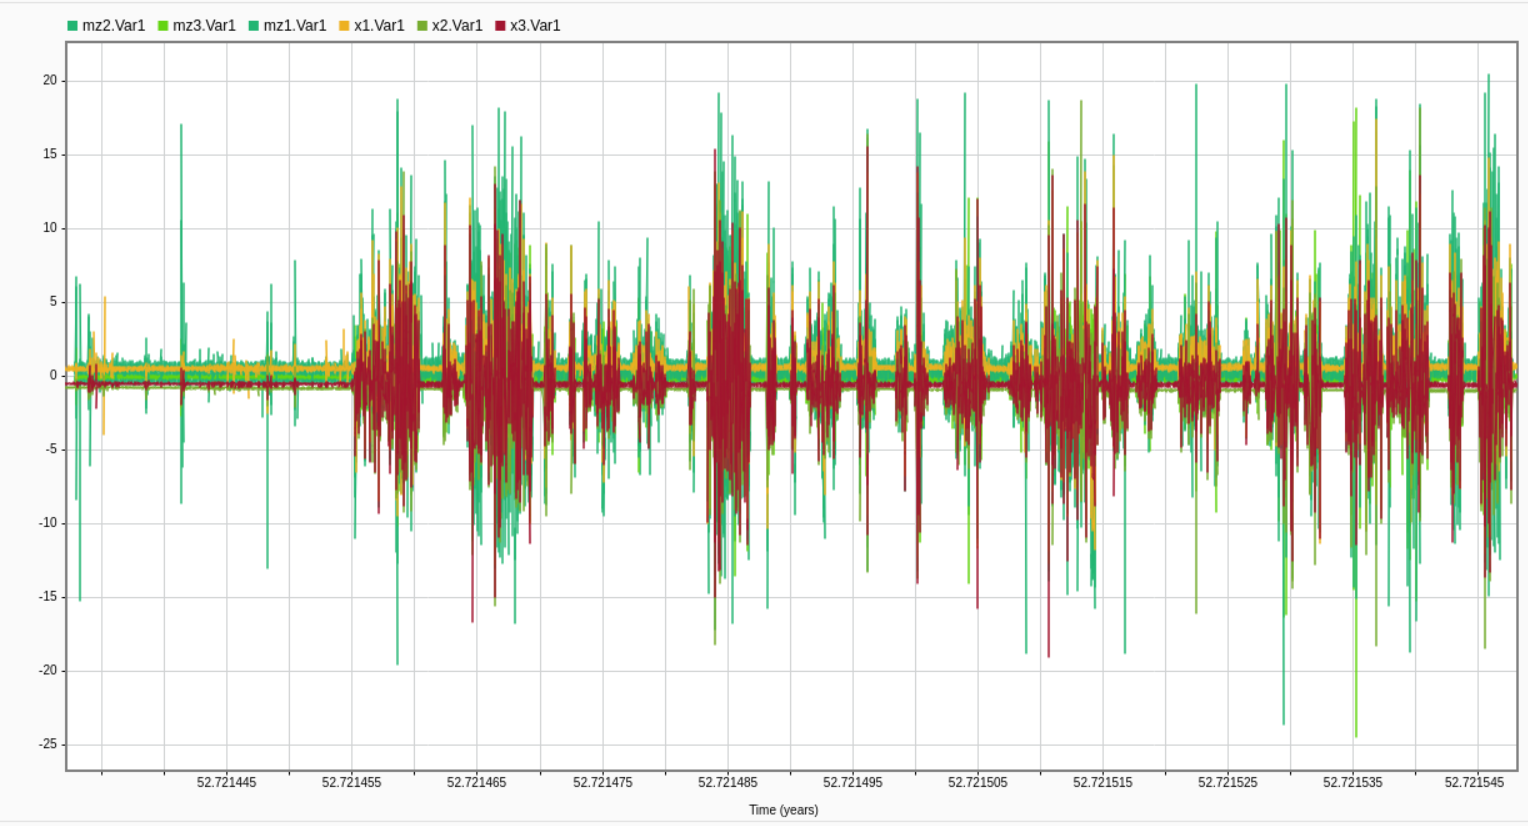
\includegraphics[width=0.85\textwidth]{chap4/figure/car_test_overall_gyro.png}
        \caption{Graph representing gyroscope data on the X axis for all the sensor boards.}
        \label{fig:car-overall-gyro}
\end{figure}

\begin{figure}[ht!]
        \centering
        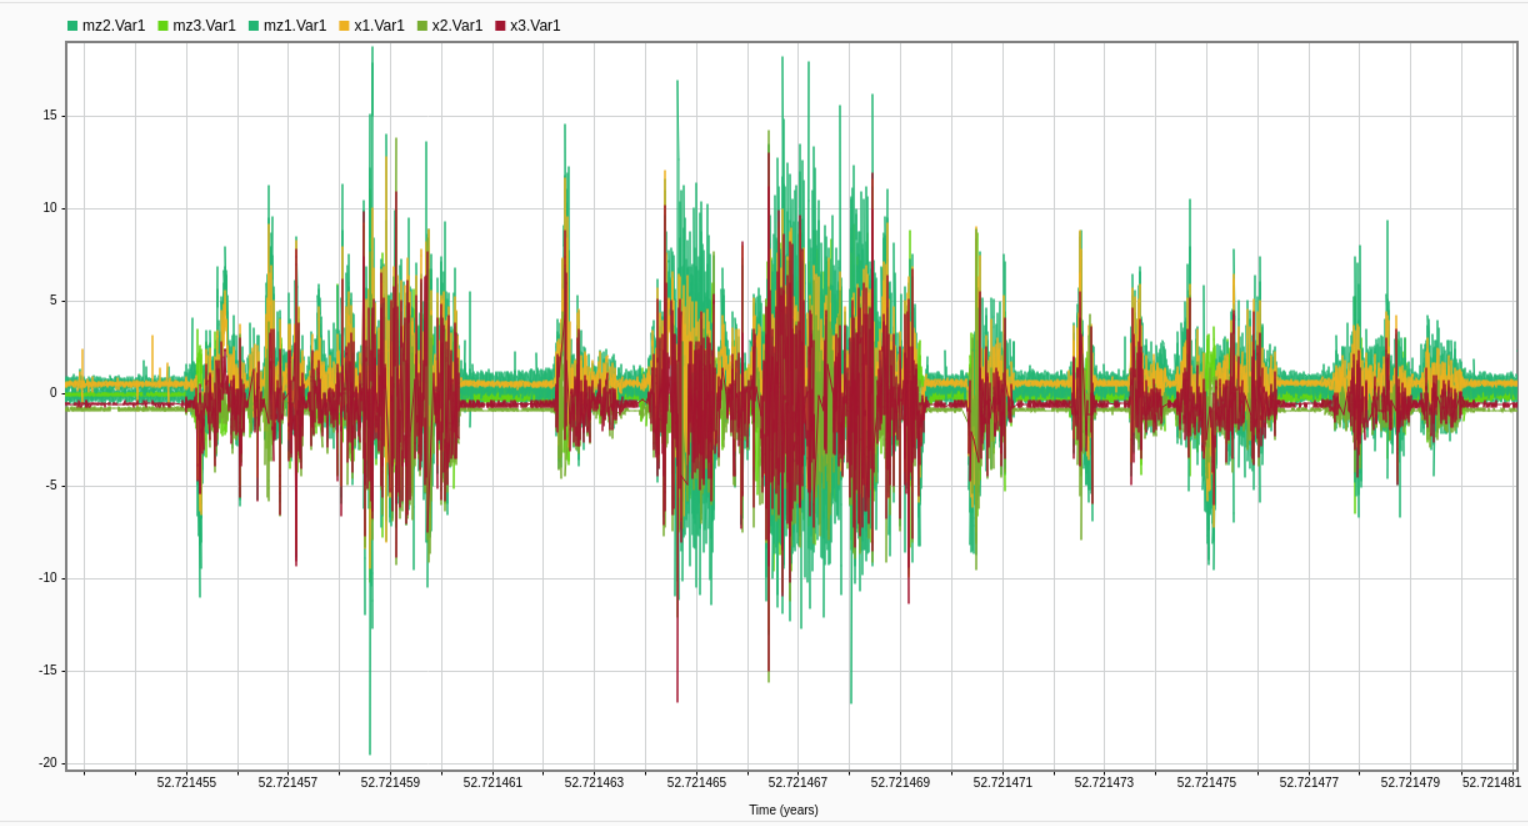
\includegraphics[width=0.85\textwidth]{chap4/figure/car_test_gyro_detail.png}
        \caption{Detail of gyroscope data.}
        \label{fig:car-detail-gyro}
\end{figure}

\FloatBarrier

Figures \ref{fig:car-overall-smartphone} and \ref{fig:car-detail-smarthpone} have been reported to show data sensed by the smartphone application compared to the sensor ones. To synchronize them over time, the clock of the smartphone (updated via Internet) have been used: it is interesting how the data coming from our sensors system is well aligned (even with a more rough precision).

\begin{figure}[ht!]
        \centering
        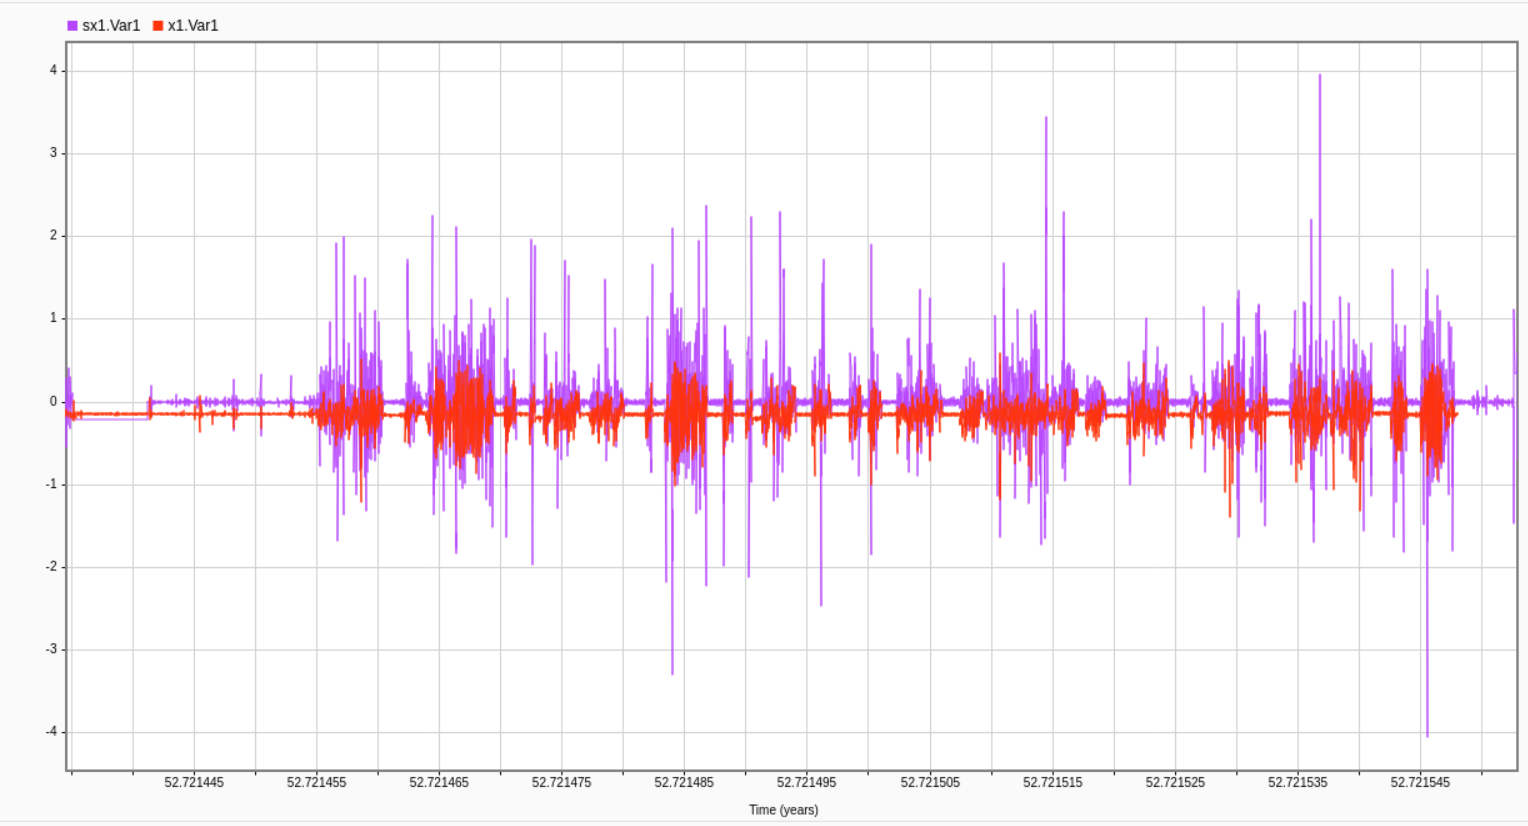
\includegraphics[width=0.85\textwidth]{chap4/figure/car_test_smartphone_overall.png}
        \caption{Graph of acceleration data from a sensor board compared to smartphone data.}
        \label{fig:car-overall-smartphone}
\end{figure}

\begin{figure}[ht!]
        \centering
        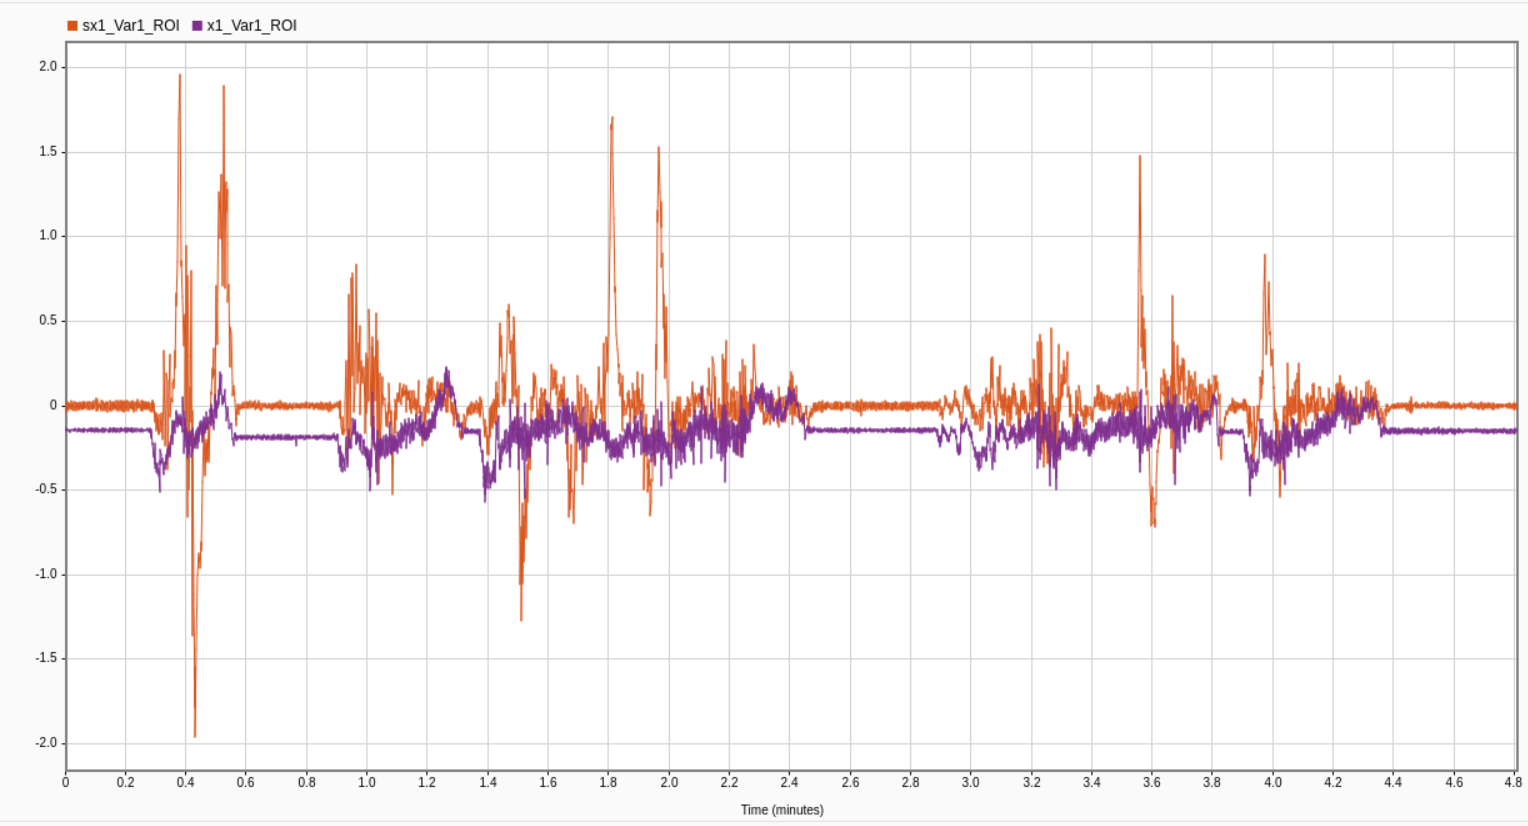
\includegraphics[width=0.85\textwidth]{chap4/figure/car_test_smartphone_detail.png}
        \caption{Detail of sensor board data compared to smartphone data.}
        \label{fig:car-detail-smarthpone}
\end{figure}

\FloatBarrier

The raw data reported until now can be corrected using the calibration algorithm explained in section 3.6. In the following images I'm reporting the results of the execution of the MATLAB script on the results coming from the sensor boards.

First, I run the calibration on the MetaMotionS (MMS) board that has been installed on the rear seat belt, as it is the one that requires more corrections.

Figure \ref{fig:mms_rawZ_calibratedY} compares the overall data between raw Z (pointing in the direction of the car) and the calibrated Y. It is evident from this image that all the samples have been moved from one axis to the other. Another detail is that the average (i.e. the acceleration of the vehicle while static) is now around 0: the offset of the raw data is removed. 

\begin{figure}[ht!]
        \centering
        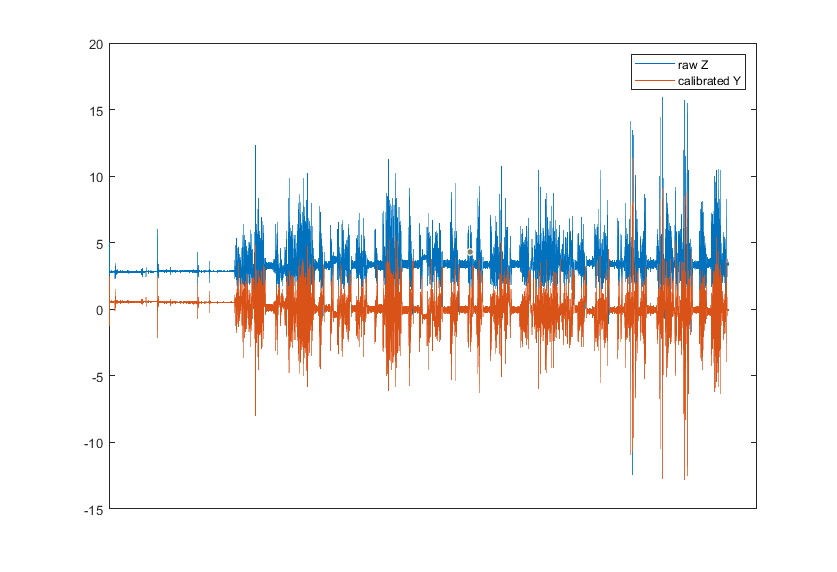
\includegraphics[width=0.85\textwidth]{chap4/figure/mms_rawZ_calibratedY.png}
        \caption{Comparison between raw data for Z axis and calibrated data for Y axis (MMS).}
        \label{fig:mms_rawZ_calibratedY}
\end{figure}

Figure \ref{fig:mms_rawZ_calibratedY_det} is a more detailed representation of the previous one. All the things said before can still be noticed, but it is also evident that the samples have been transferred symmetrically around the horizontal axis of the graph: this is because the axis of the sensor that was pointing to the car movement was 180° rotated.

\begin{figure}[ht!]
        \centering
        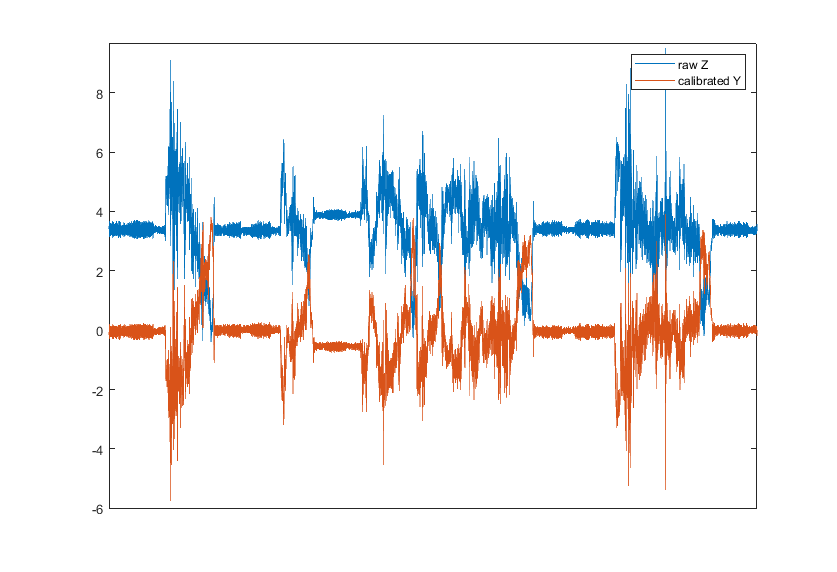
\includegraphics[width=0.8\textwidth]{chap4/figure/mms_rawZ_calibratedY_detail.png}
        \caption{Detail of the comparison between raw data for Z axis and calibrated data for Y axis (MMS).}
        \label{fig:mms_rawZ_calibratedY_det}
\end{figure}

Figure \ref{fig:mms_rawX_calibratedX} compares the raw and calibrated data for the X axis. The X axis was the one pointing to ground, so raw data contained the gravity acceleration. Calibrated data is representing, instead, the real acceleration on the X axis, so there is no gravity component. 

\begin{figure}[ht!]
        \centering
        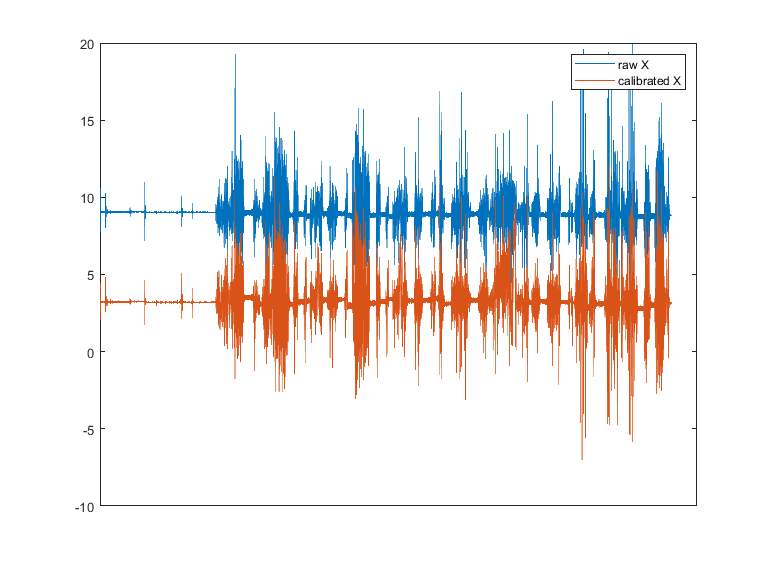
\includegraphics[width=0.8\textwidth]{chap4/figure/mms_rawX_calibratedX.png}
        \caption{Comparison between raw data for X axis and calibrated data for the same axis (MMS).}
        \label{fig:mms_rawX_calibratedX}
\end{figure}
\FloatBarrier
Figure \ref{fig:mms_rawY_calibratedY} compares raw and calibrated data for Y axis. Also in this case, due to rotation, the data represented in the calibrated version is composed of different components from the axis, so original and elaborated samples are not dependent. 

\begin{figure}[ht!]
        \centering
        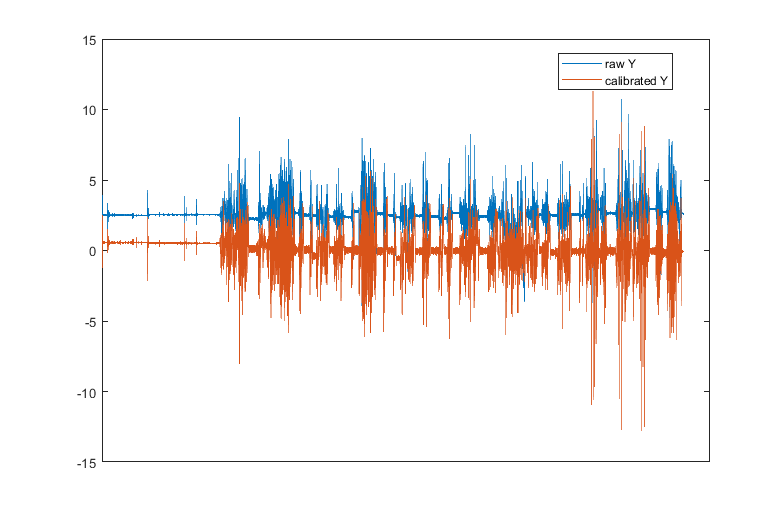
\includegraphics[width=0.7\textwidth]{chap4/figure/mms_rawY_calibratedY.png}
        \caption{Comparison between raw data for Y axis and calibrated data for the same axis (MMS).}
        \label{fig:mms_rawY_calibratedY}
\end{figure}

Figure \ref{fig:mms_rawZ_calibratedZ} compares raw and calibrated data for Z axis. The calibrated samples average to 9.81, that is the gravity acceleration: it has been moved from the X axis to this one. 

\begin{figure}[ht!]
        \centering
        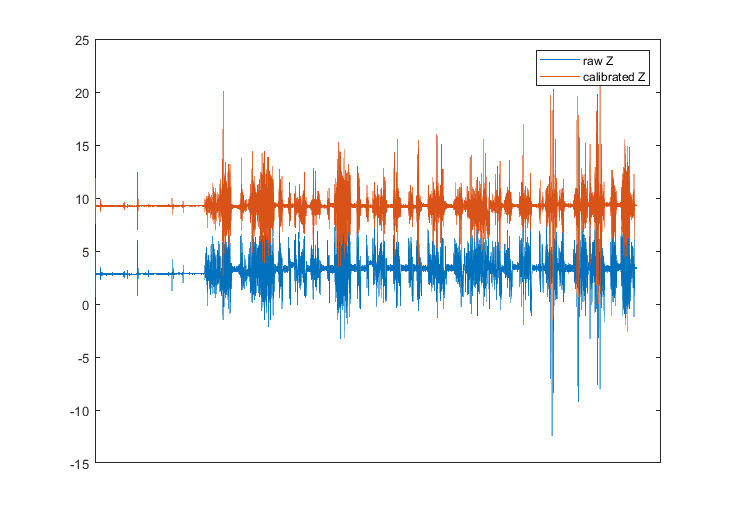
\includegraphics[width=0.65\textwidth]{chap4/figure/mms_rawZ_calibratedZ.png}
        \caption{Comparison between raw data for Z axis and calibrated data for the same axis (MMS).}
        \label{fig:mms_rawZ_calibratedZ}
\end{figure}

\FloatBarrier

Then, I performed the calibration on the results of one of the ST sensors. They were correctly positioned with regards to the Z axis, but the X and Y axis would require some rotation. 

Figure \ref{fig:st_rawZ_calibratedZ} reports calibrated data for the Z axis compared to the raw one. Values are the same, but calibrated one is mirrored with respect to the horizontal axis.
\begin{figure}[ht!]
        \centering
        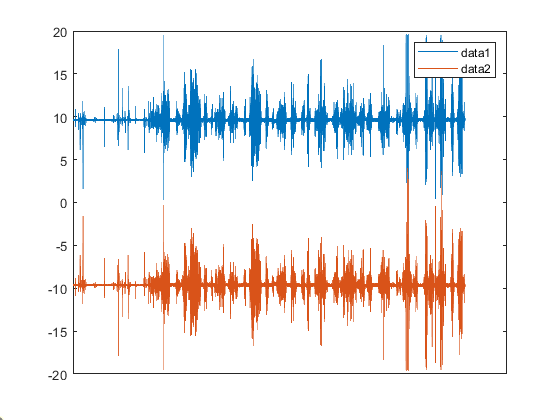
\includegraphics[width=0.8\textwidth]{chap4/figure/st_rawZ_calibratedZ.png}
        \caption{Comparison between raw data for Z axis and calibrated data for the same axis (ST).}
        \label{fig:st_rawZ_calibratedZ}
\end{figure}

\FloatBarrier

Figure \ref{fig:st_rawX_calibratedY} compares raw X data and calibrated Y data. They represent the same values, as originally the sensor had its X axis coherent with the car movement, but the calibration algorithm moved those acceleration components on the Y axis.

\begin{figure}[ht!]
        \centering
        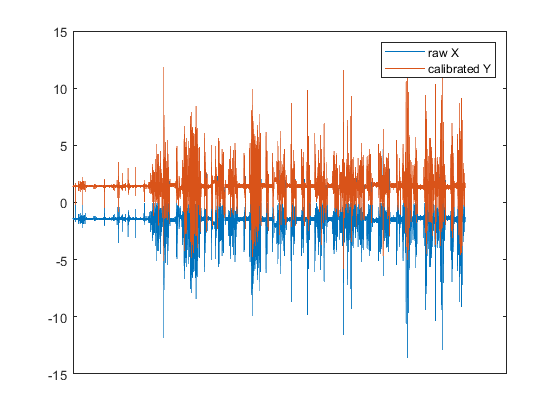
\includegraphics[width=0.8\textwidth]{chap4/figure/st_rawX_calibratedY.png}
        \caption{Comparison between raw data for X axis and calibrated data for the Y axis (ST).}
        \label{fig:st_rawX_calibratedY}
\end{figure}

Figure \ref{fig:st_rawX_calibratedY_det} is a detail of the previous one and it shows that also in this case data is mirrored: in this way, the acceleration of the car is positive after staying steady. Raw data (in blue) represents negative acceleration in all cases, but it doesn't make sense, as the car didn't go reverse.

\begin{figure}[ht!]
        \centering
        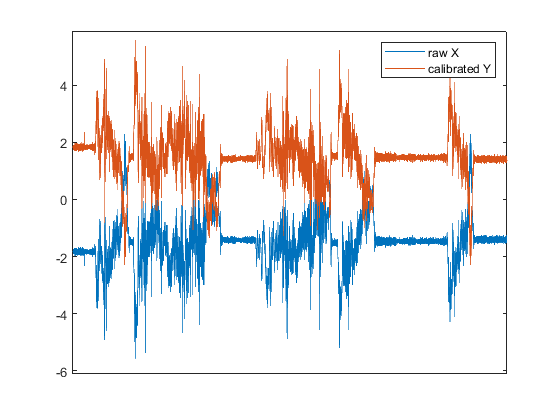
\includegraphics[width=0.8\textwidth]{chap4/figure/st_rawX_calibratedY_detail.png}
        \caption{Detail of the comparison between raw data for X axis and calibrated data for the Y axis (ST).}
        \label{fig:st_rawX_calibratedY_det}
\end{figure}

\FloatBarrier

Figures \ref{fig:st_rawY_calibratedX} and \ref{fig:st_rawY_calibratedX_det} both show comparison between raw Y and calibrated X. Also in this case, data from Y axis is moved on the X one, as the algorithm is designed in this way, but it's also mirrored: this happens because, when rotating the sensor axis 90 degrees (to bring X acceleration on Y axis), also the other component is rotated, causing it to be the negative of the original one. 

\begin{figure}[ht!]
        \centering
        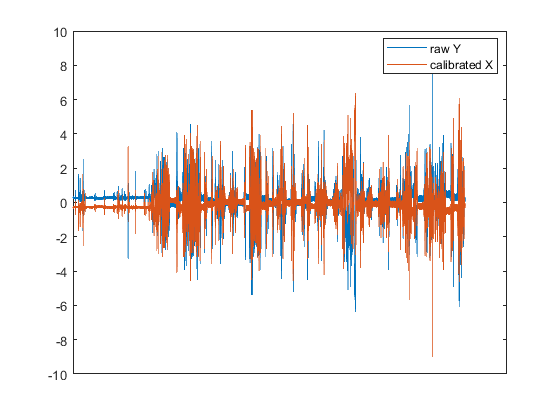
\includegraphics[width=0.8\textwidth]{chap4/figure/st_rawY_calibratedX.png}
        \caption{Comparison between raw data for Y axis and calibrated data for the X axis (ST).}
        \label{fig:st_rawY_calibratedX}
\end{figure}

\begin{figure}[ht!]
        \centering
        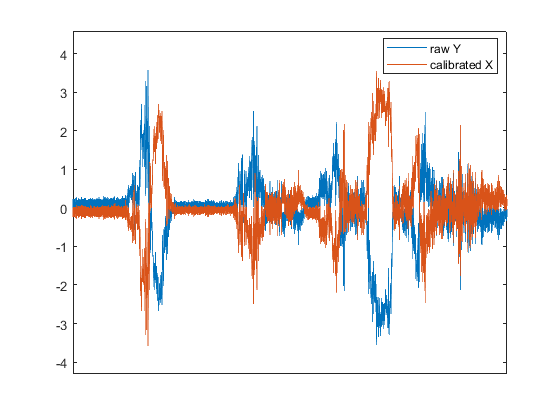
\includegraphics[width=0.8\textwidth]{chap4/figure/st_rawY_calibratedX_detail.png}
        \caption{Detail of comparison between raw data for Y axis and calibrated data for the X axis (ST).}
        \label{fig:st_rawY_calibratedX_det}
\end{figure}

\FloatBarrier

To show the potential of the acquisition system, I prepared some videos combining the data acquired from IMUs and the images acquired by the video camera. In this case, the synchronization between the two was not immediate, as the video shooting is not considered in the time synchronization mechanism: it required some manual adjustment. In any case, the video had the current time (obtained from GPS data) superimposed, and thanks to the MATLAB timetables structures generated from the elaboration scripts, finding the corresponding sample (with 1 second accuracy) has been quite easy. Then, thanks to the MATLAB \textit{VideoWriter} functionality, I created an animation that can be easily integrated to the shot images thanks to a video editing program, like DaVinci Resolve 18 by BlackMagic \cite{davinciresolve}. A snapshot of the result is reported in Figure \ref{fig:snapshot-from-video}, and I'm reporting some conclusions on the experiment in the following paragraphs.

\begin{figure}[ht!]
        \centering
        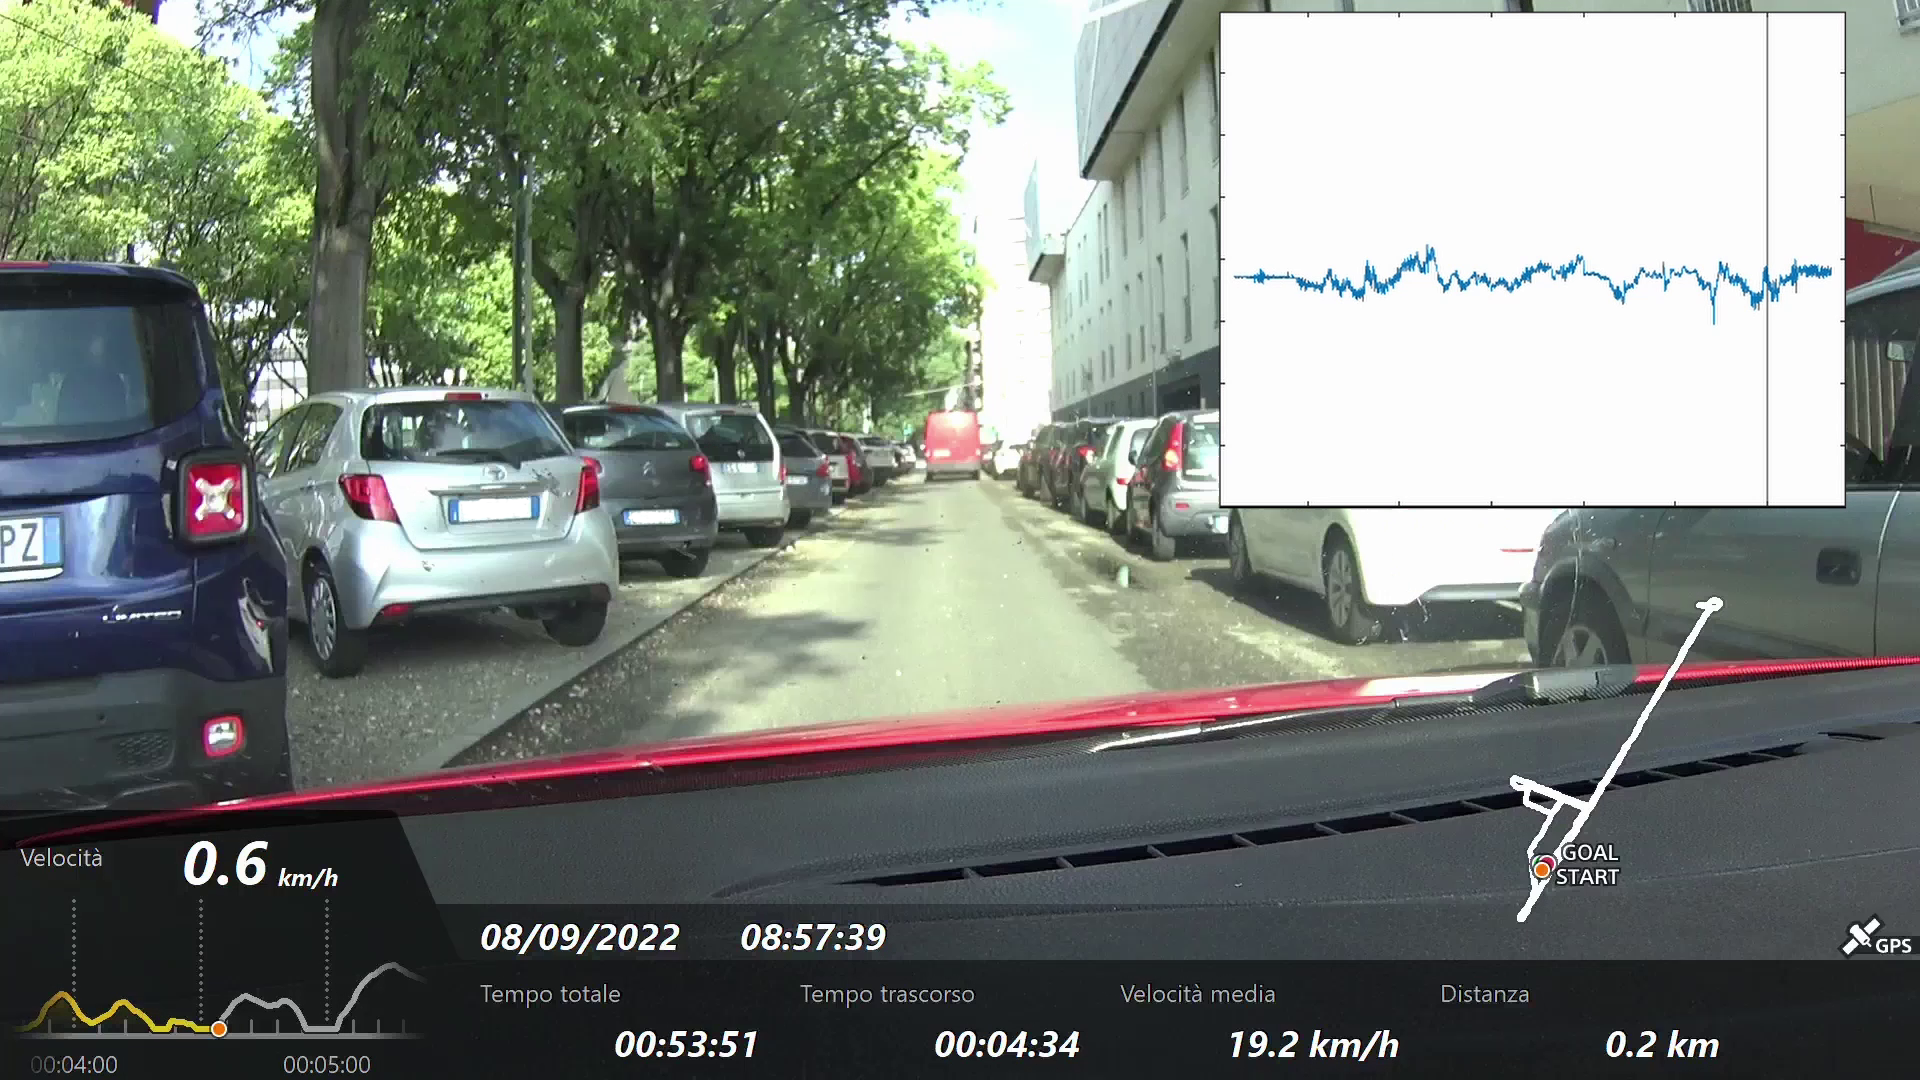
\includegraphics[width=0.85\textwidth]{chap4/figure/vlcsnap1.png}
        \caption{Snapshot from the final video with both images and IMU data.}
        \label{fig:snapshot-from-video}
\end{figure}

\paragraph{Overall behaviour of the system} The system demonstrated strong reliability during the experiment, as no disconnection happened and the stream of data worked continuously all the time (around 1 hour). The fetched data is coherent with all the different devices inside my system, and comparing them with the samples of an external device (the smartphone) gave good results. Time synchronization worked as expected for all the duration of the experiment, keeping the same performance as in section 4.2.

\paragraph{Board positioning} It is important to put the sensor boards accurately in the car, choosing stiff points in which vibrations are limited. For example, fixing the boards on the dashboard with adhesive tape is a good idea, as data coming from the ST devices is clean and coherent. Also the clip accessories for MetaMotionS are a good idea, but they shouldn't be put on the seat belt or other moving parts, as the motion data is compromised (Figure \ref{fig:car-detail2-acc}). During the sensors installation, it is also important to remember the axis direction, but anyway an appropriate calibration algorithm is enough to fix it.

\paragraph{Data elaboration} As explained for Figure \ref{fig:car-detail1-acc} in particular, it's important to consider the differences between the sensors during data elaboration in Matlab. In this case, it could be convenient to remove the offset from all the devices data, to set the steady state around the value 0 (and not -0.3). It would be also a good idea to analyze the positioning of the sensors and align correctly the data (in this case, it simply means to put a minus to the mz3 values). 

\paragraph{Audio and Frequencies} The main idea behind the analysis of audio frequencies was to automatically label all the events using these values. Figure \ref{fig:car-detail-freqacc} shows that this can be possible, even if Figure \ref{fig:car-overall-freqacc} is proof that, in this experiment, this solution needs some further analysis. In particular, it seems that lower frequencies are not distinguishable from the background noises, and other frequencies are not shown probably because they were not the dominant ones. Possible solutions can be:
\begin{itemize}
    \item Use higher frequencies, that seem to be recognized more easily
    \item Do some experiments in car with the same sensors, maybe with real-time results on the computer screen, to understand which frequencies are better to use.
    \item Put the speaker of the audio frequency generator nearer to the sensor microphone.
    \item Analyze more dominant frequencies than the first. In this case, only the frequency with the maximum power spectrum have been considered: maybe taking also the second and the third one could be beneficial in finding the reproduced ones. 
    \item Make the car environment better for the noise propagation (for example, close all windows, put sensors on different parts of the car that don't vibrate and so on).
\end{itemize}
Another problem we noticed during the experiment is that programming the audio frequency to be played on the Android app is not easy. Every time, the old value should be deleted, the new one should be written, and so on. This procedure is slow and error-prone. An idea could be to pre-record audio data at certain frequencies, and use those audio files. In this way, the time duration of the sound is already known, the user is not confused between different frequency values and at the same time the correct one can be played without hassle.  
